\documentclass[letterpaper,10pt]{article}

\usepackage{titling}
\usepackage{listings}
\usepackage{url}
\usepackage{setspace}
\usepackage{subfig}
\usepackage{sectsty}
\usepackage{pdfpages}
\usepackage{colortbl}
\usepackage{multirow}
\usepackage{multicol}
\usepackage{relsize}
\usepackage{amsmath}
\usepackage{fancyvrb}
\usepackage[yyyymmdd]{datetime}
\usepackage{amsmath,amssymb,amsthm,graphicx,xspace}
\usepackage[titlenotnumbered,noend,noline]{algorithm2e}
\usepackage[compact]{titlesec}
\usepackage{XCharter}
\usepackage[T1]{fontenc}
\usepackage{tikz}
\usetikzlibrary{arrows,automata,shapes,trees,matrix,chains,scopes,positioning,calc}
\tikzstyle{block} = [rectangle, draw, fill=blue!20, 
    text width=2.5em, text centered, rounded corners, minimum height=2em]
\tikzstyle{bw} = [rectangle, draw, fill=blue!20, 
    text width=4em, text centered, rounded corners, minimum height=2em]

\definecolor{namerow}{cmyk}{.40,.40,.40,.40}
\definecolor{namecol}{cmyk}{.40,.40,.40,.40}
\renewcommand{\dateseparator}{-}


\let\LaTeXtitle\title
\renewcommand{\title}[1]{\LaTeXtitle{\textsf{#1}}}


\newcommand{\handout}[5]{
  \noindent
  \begin{center}
  \framebox{
    \vbox{
      \hbox to 5.78in { {\bf ECE252: Systems Programming and Concurrency } \hfill #2 }
      \vspace{4mm}
      \hbox to 5.78in { {\Large \hfill #4  \hfill} }
      \vspace{2mm}
      \hbox to 5.78in { {\em #3 \hfill \today } }
    }
  }
  \end{center}
  \vspace*{4mm}
}

\newcommand{\lecture}[3]{\handout{#1}{#2}{#3}{Lecture #1}}{
\newcommand{\tuple}[1]{\ensuremath{\left\langle #1 \right\rangle}\xspace}

\addtolength{\oddsidemargin}{-1.000in}
\addtolength{\evensidemargin}{-0.500in}
\addtolength{\textwidth}{2.0in}
\addtolength{\topmargin}{-1.000in}
\addtolength{\textheight}{1.75in}
\addtolength{\parskip}{\baselineskip}
\setlength{\parindent}{0in}
\renewcommand{\baselinestretch}{1.5}
\newcommand{\term}{Spring 2019}

\singlespace


\begin{document}

\lecture{ 27 --- Concurrency in File Systems }{\term}{Jeff Zarnett}

\section*{Concurrency in File Systems}

To understand the idea of concurrency in file systems, we need to peel back the interface a bit and have at least a high-level understanding of their implementation. File can be of arbitrary size (although in a particular file system there may be a limit), so they have to be allocated on disk according to some strategy.

The contiguous allocation strategy means that a file occupies a set of contiguous blocks on disk. So a file is allocated, starting at block $b$ and is $n$ blocks in size, the file takes up blocks $b, b+1, b+2, ..., b+(n-1)$. But for a sufficiently large file, it might be difficult to find a place to put it. And we also don't know how to predict the size of a file, so how much space do we leave for where to put it?

Linked allocation is a solution to the problems of contiguous allocation: instead of a file being all in consecutive blocks, we maintain a linked list of the blocks, and the blocks themselves may be located anywhere on the disk. The directory listing just has a pointer to the first and last blocks (head and tail of the linked list). Unfortunately, however, accessing block $i$ of a file is no longer as simple as computing an offset from the first block; it requires following $i$ pointers (a pain). If we want to go to the middle of a file, why do we have to load every block on the way there?

There's a compromise approach: indexed allocation. The idea of indexed allocation is to take all the pointers and put them into one location: an index block. So, the first block of the file contains a whole bunch of pointers. To get to block $i$, just go to index $i$ of the index block and we can get the location of block $i$ much more efficiently than we could in linked allocation. All pointers to blocks start as null, and when we add a new block, add its corresponding entry into the index block~\cite{osc}. See the diagram below:

\begin{enumerate}
	\item \textbf{Linked Scheme}: An index block is a disk block, and we can link together several index blocks. The last entry in the index block is either null or a pointer to the next index block.
	\item \textbf{Multilevel Index}: A variant of the linked scheme that has multiple levels. The first level block points to the second level block; the second level block points to the actual file data. This can go to as many levels are necessary based on the maximum file size. If a block is 4~KB, we can have 1024 4-byte pointers, so two levels would allow a maximum file size of up to 4~GB.
	\item \textbf{Combined Scheme}: The all-of-the-above option. This is used in UNIX. Keep the first 15 pointers of the index block in the inode structure; 12 of them point directly to file data. The next three pointers refer to indirect blocks. The 13th is an index block containing the addresses of blocks with data. The 14th points to a double indirect block (addresses of blocks containing addresses of blocks). The 15th points to a triple indirect block\footnote{Yo dawg, we heard you like index blocks...}.
\end{enumerate}

With that out of the way, we can show a visual representation of an inode. This is just another sort of data structure, except it is stored in persistent storage. It will be helpful to keep this in mind. When we lock a file, implicitly we need to know which inode we are locking.

\begin{center}
	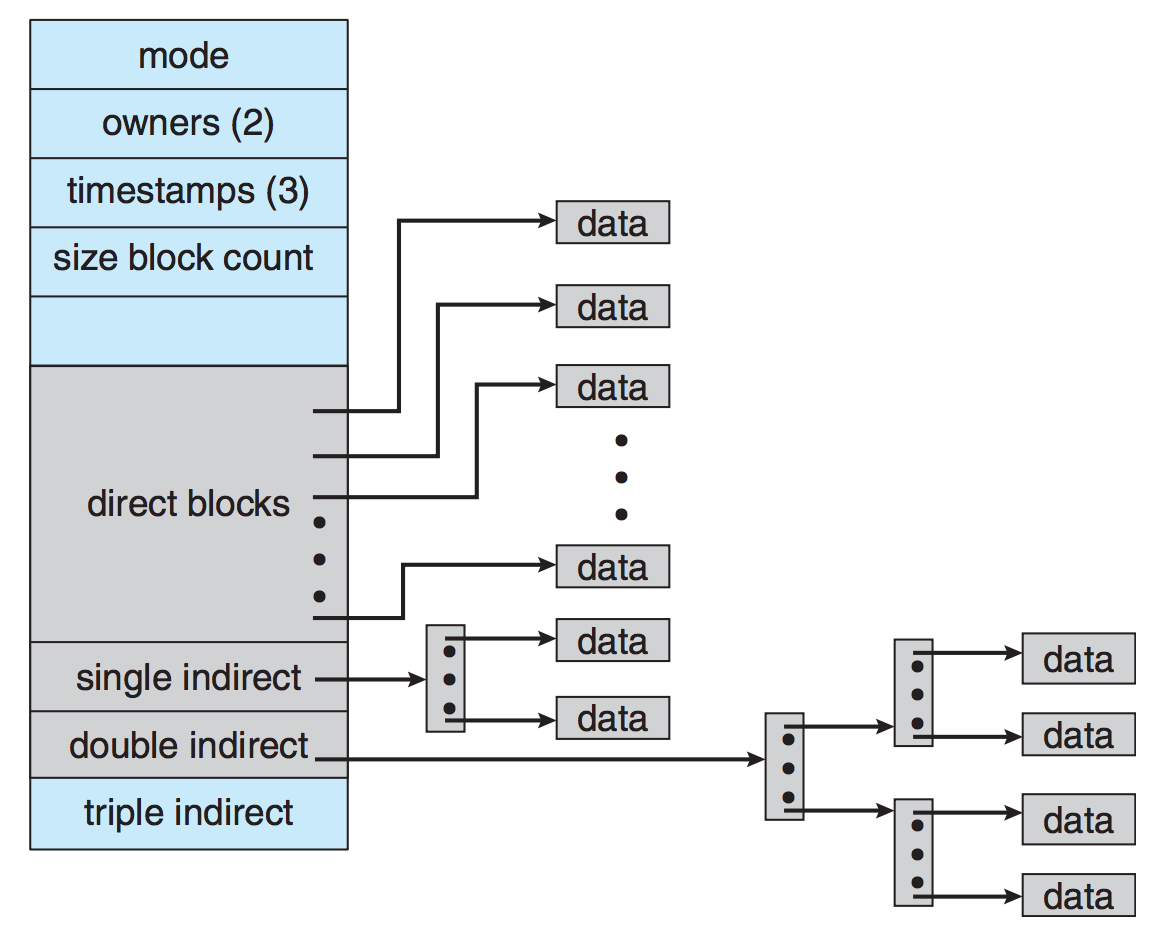
\includegraphics[width=0.6\textwidth]{images/unix-inode.png}\\
	The UNIX inode. Triple indirection is left to the reader's imagination~\cite{osc}.
\end{center}

We already discussed the use of \texttt{flock()} to lock a file, and this locks the entire file. There exists another way to lock a file, using \texttt{fcntl}, in which case we can lock only a part of a file, specifically a byte range of that file. This is referred to as \textit{record locking}.

Locking just a part of the file allows for more concurrency: if a process is writing the beginning of the file, another one can be writing the end of the file and these don't overlap so the second write does not need to wait. Let's see how to do that. The function is found in the header \texttt{fcntl.h}. Here's the function signature:

\begin{lstlisting}[language=C]
int fcntl( int file_descriptor, int command, ... /* struct flock * flockptr */ )
\end{lstlisting}

This one looks strange! It turns out that \texttt{fcntl} can do a lot of things, and only sometimes the third argument is needed. So it is a \texttt{...} (list of args) but we would only fill it with one \texttt{struct flock} if we need to based on the value of \texttt{command}. They could have just overloaded this function, but, well, here we are.

The \texttt{struct flock} has the following definition~\cite{apunix}:
\begin{lstlisting}[language=C]
struct flock {
  short  l_type;   /* F_RDLCK, F_WRLCK, or F_UNLCK */
  short  l_whence; /* SEEK_SET, SEEK_CUR, or SEEK_END */
  off_t  l_start;  /* offset in bytes, relative to l_whence */
  off_t  l_len;    /* length, in bytes; 0 means lock to EOF */
  pid_t  l_pid;    /* returned with F_GETLK */
};
\end{lstlisting}

Much like the readers-writers locks, the types of locks are read and write. The compatibility matrix is exactly what you would expect: read locks are compatible with other read locks; write locks are not compatible with any other lock. And finally, to unlock, you still use the set-lock functionality, but with type \texttt{F\_UNLCK}. This sort of locking scheme is vulnerable to deadlock, as it's possible for a process to lock file 1 and need file 2 while another process has a lock on file 2 and needs the lock on file 1.

The value of \texttt{l\_whence} is going to be one of the three constants named in the comment above. This refers to where the offset begins. \texttt{SEEK\_SET} means at the start of the file. So if you specify \texttt{SEEK\_SET} and an offset of \texttt{1000} it means the locked region begins 1000 bytes after the start of the file. \texttt{SEEK\_END} means the relative point is the end of the file. Finally, \texttt{SEEK\_CUR} means based on the current position in the file (if you've positioned within the file using \texttt{seek()} this makes sense).

It is possible for a locked region to extend past the end of the file. This is used when appending to the file, so you don't have to know in advance how much you plan to append to the file. If 0 is given for the length that does include anything appended to the file as well.


For \texttt{command}, our choices are~\cite{apunix}:
\begin{itemize}
	\item \texttt{F\_GETLK} -- Determine if the lock described by \texttt{flockptr} is blocked by some other lock. If a lock exists, the content of \texttt{flockptr} is overwritten with the data of the lock; if no lock exists then the \texttt{l\_type} field is set to \texttt{F\_UNLCK}.
	\item \texttt{F\_SETLK} -- Set the lock as described by \texttt{flockptr}. If the lock cannot be acquired then the return value of the function returns an error and \texttt{errno} are set. This is ``trylock''-behaviour and can be used to avoid the possibility of a deadlock.
	\item \texttt{F\_SETLKW} -- A blocking version of the \texttt{F\_SETLK} command. If the region we want to lock is currently in use then the caller gets blocked.
\end{itemize}

When unlocking a region, just as for locking, you can specify what part of the file you would like to unlock. Partial unlocking is unusual, but why not? The system will combine or split locks as appropriate, based on what is to be locked or unlocked.

Let's do some examples on how to use this structure and system call. The first example is how to lock a file and then how to unlock it:

\begin{lstlisting}[language=C]
int write_lock_file( int fd ) {

  struct flock fl;
  fl.l_type = F_WRLOCK;
  fl.l_start = 0;
  fl.l_whence = SEEK_SET;
  fl.l_len = 0;
  
  return fcntl( fd, F_SETLK, &fl );
}

int unlock_file( int fd ) {

  struct flock fl;
  fl.l_type = F_UNLCK;
  fl.l_start = 0;
  fl.l_whence = SEEK_SET;
  fl.l_len = 0;
  
  return fcntl( fd, F_SETLK, &fl );
}
\end{lstlisting}

Obviously if you wished to have a different type of lock or to only lock a specific range, then you would need different values in the structure. Now for checking if a given part of a file is locked:

\begin{lstlisting}[language=C]
int fd = open ( "example.txt", O_RDONLY );
struct flock lock;

lock.l_type = F_RDLOCK;
lock.l_start = 1024;
lock.l_whence = SEEK_SET;
lock.l_len = 256;

fcntl( fd, F_GETLK, &lock );
if ( lock.l_type == F_UNLCK ) {
	/* Lock is unlocked; we may proceed */
} else if ( lock.l_type = F_WRLOCK ) {
  /* File is write locked by a different process */
  printf( "File locked by process ID %d.\n", lock.l_pid );
  return -1;
}
\end{lstlisting}

Checking on things with \texttt{F\_GETLK} is really for information purposes only: you should not make decisions about whether to proceed based on this, because of course the sequence of ``read of the value and then whatever operation you'd like to do next'' is not atomic. Instead, use the command \texttt{F\_SETLK} and actually try to set the lock. If \texttt{-1} is returned then locking was not successful. Or, if the plan is to wait, use \texttt{F\_SETLKW} as one would expect.

It's important to remember that \texttt{fcntl} changes some values of the \texttt{struct lock} so if you wanted to re-use it you need to make sure to reset it as appropriate. You can use the same \texttt{struct lock} later to unlock the thing that you locked, just do so carefully.

I'll also take a minute to mention \texttt{lockf}: it is a simplified way of locking a file. While \texttt{fcntl} is more flexible, sometimes all we need is the simple version. According to the documentation:

\begin{lstlisting}[language=C]
int lockf( int file_descriptor, int command, off_t length );
\end{lstlisting}

The command options can be:
\begin{itemize}
	\item \texttt{F\_LOCK} -- Acquire an exclusive lock on the (section of the) file.
	\item \texttt{F\_TLOCK} -- Try to acquire an exclusive lock (try-lock behaviour).
	\item \texttt{F\_ULOCK} -- Unlock the indicated section of the file.
	\item \texttt{F\_TEST} -- Check if (a section of) the file is locked; 0 if it is unlocked and -1 if the file is locked.
\end{itemize}


The length is an offset, and is based off the current position in the file. If zero is provided then it locks the whole file.

Two further notes: The file is automatically unlocked when the file descriptor is closed. And, on some systems \texttt{lockf} just calls \texttt{fcntl} but on some others they use different mechanisms. So don't mix and match. If you lock a file with one function, unlock it with the matching one.

It is noteworthy that both kinds of lock are ``advisory'' only. That is, like the use of a semaphore or mutex, it only is really effective if everyone involved in accessing the shared resource follows the proper protocol and checks if access is permitted or not. Mandatory locks do exist, but are hard to use and are not recommended. Did you really want to know about mandatory locking? Well, check out this kernel.org documentation as to why you shouldn't, but also how it works if you must: \url{https://www.kernel.org/doc/Documentation/filesystems/mandatory-locking.txt}.

\subsection*{Using A File as a Lock}

We can use the very existence of a file as a way of controlling concurrency. For example, \texttt{git} places a file \texttt{index.lock} in a particular directory to indicate that an operation is in progress so two different \texttt{git} clients do not operate on the same repository at the same time. So that is one strategy: check if the file is present; if it is, the resource is ``locked'', if no such file is present then it is ``unlocked''.

If we want to check, we just try to \texttt{open()} the file, but unless we are careful this can lead to a problem if two processes want to create the file: if they both call \texttt{open}, they both might succeed. To get around this, we need to use the \texttt{flags} parameter of the call to open the file. See below.

\begin{lstlisting}[language=C]
int open(const char *filename, int flags);  /* Returns a file descriptor if successful, -1 on error */
int rename(const char *old_filename, const char *new_filename); /* Returns 0 on success , operates atomically */
int remove(const char *filename) ; /* Deletes a file or directory, returns 0 on success, operates atomically */ 
\end{lstlisting}

When opening a file the following flags may be used for the \texttt{flags} parameter (and can be combined with bitwise OR, the \texttt{|} operator):

\begin{tabular}{l|l}
	\textbf{Value}     & \textbf{Meaning}                                                                                 \\ \hline
	\texttt{O\_RDONLY} & Open the file read-only                                                                          \\ \hline
	\texttt{O\_WRONLY} & Open the file write-only                                                                         \\ \hline
	\texttt{O\_RDWR}   & Open the file for both reading and writing                                                       \\ \hline
	\texttt{O\_APPEND} & Append information to the end of the file                                                        \\ \hline
	\texttt{O\_TRUNC}  & Initially clear all data from the file                                                           \\ \hline
	\texttt{O\_CREAT}  & Create the file                                                                                  \\ \hline
	\texttt{O\_EXCL}   & If used with \texttt{O\_CREAT}, the caller MUST create the file; if the file exists it will fail \\
\end{tabular}

We can combine the use of \texttt{open} with \texttt{rename} to get lock-like behaviour between different programs that share nothing except a common file system. The \texttt{open} call should be used to create the lock file, and fail if the file already exists. If we want we can use \texttt{remove} to delete the lock file if we want to let the next process try, but there's an alternative option: \texttt{rename}.

Because the \texttt{rename} function is also atomic, we can use it too, and just rename the existing lock file rather than creating it and deleting it every time. Then programs that want their turn should use \texttt{rename}; if a process or thread does succeed in renaming the file it is that process or thread's turn; otherwise, they have to wait. To unlock, just change the name back. Consider this simple example that uses threads (rather than processes):

\begin{lstlisting}[language=C]
#include <stdio.h>
#include <stdlib.h>
#include <fcntl.h>
#include <unistd.h>
#include <sys/stat.h>
#include <sys/types.h>
#include <pthread.h>

#define NUM_THREADS 10

int lock_fd;
int shared = 0;

void* run( void* arg ) {
  int* id = (int*) arg;
  while( rename( "file.lock", "file.locked" ) == -1 ) {
    printf("Thread %d waiting.\n", *id); 
  }

  printf("Thread %d in critical section.\n", *id);
  printf("Shared incremented from %d", shared);
  shared++;
  printf(" to %d.\n", shared);
  rename("file.locked", "file.lock"); /* Unlock */

  free( arg );
  pthread_exit(NULL);
}

void* writer( void* arg ) {
  /* Write data implementation not shown */
  pthread_exit(NULL);
}


int main( int argc, char** argv ) {
  lock_fd = open( "file.lock", O_CREAT | O_EXCL );  
  if (lock_fd == -1 ) {
   printf( "File creation failed.\n");
   return -1;
  }

  pthread_t threads[NUM_THREADS];
  for (int i = 0; i < NUM_THREADS; i++) {
    int * id = malloc( sizeof( int ) );
    *id = i;
    pthread_create( &threads[i], NULL, run, id );
  }
  for (int i = 0; i < NUM_THREADS; i++) {
    pthread_join( threads[i], NULL );
  }
  close( lock_fd );
  remove( "file.lock" );

  return 0;
}
\end{lstlisting}

\bibliographystyle{alphaurl}
\bibliography{252}


\end{document}